\chapter{Testing}

%Testing is a fundamental phase in the developing process of an embedded system. It is important to define test plan at each level of design and is necessary to test not only the software but also if the global system matches all the specified requirements.

We will now show a subset of all tests that have been performed on the system. 

Through all phases of system development, several tests have been performed, either on hardware or software components, which involved both prototypes and final system implementation. Main tests on the system involved real use case scenarios, e.g.\ observing system's reactions to obstacles in sonar's field of vision at different distances and angles, providing hence the system a various set of different inputs.

Apart from these tests, individual software components have also been tested using {\em CUnit} suite, performing functional and conformance testing. According to what is required by the committee, only these latter tests are illustrated in following sections.


\section{Conformance Tests}

This section illustrates tests performed by the first suite included in our automatic testing program. This suite performs conformance testing of a state machine that is included inside Sensor module used to manage erroneous states the system can get into after partial or total hardware failures. These erroneous states are all identified depending on each sensor's echo response width, as shown in Figure \ref{fig:echo_widths}. In the Figure, arrows represent two consecutive activations of Step Task.






\begin{figure}[tp]
\centering
\subfloat[Correct sensor behavior, next state will be State OK and trigger signal can be sent again at next activation]{\includegraphics[width=0.8\textwidth]{tikz_img/trig_echo_ok.eps}\label{fig:state_ok}}\\

\subfloat[Stuck at zero echo behavior, next state will be State Lost and trigger signal can be sent again at next activation]{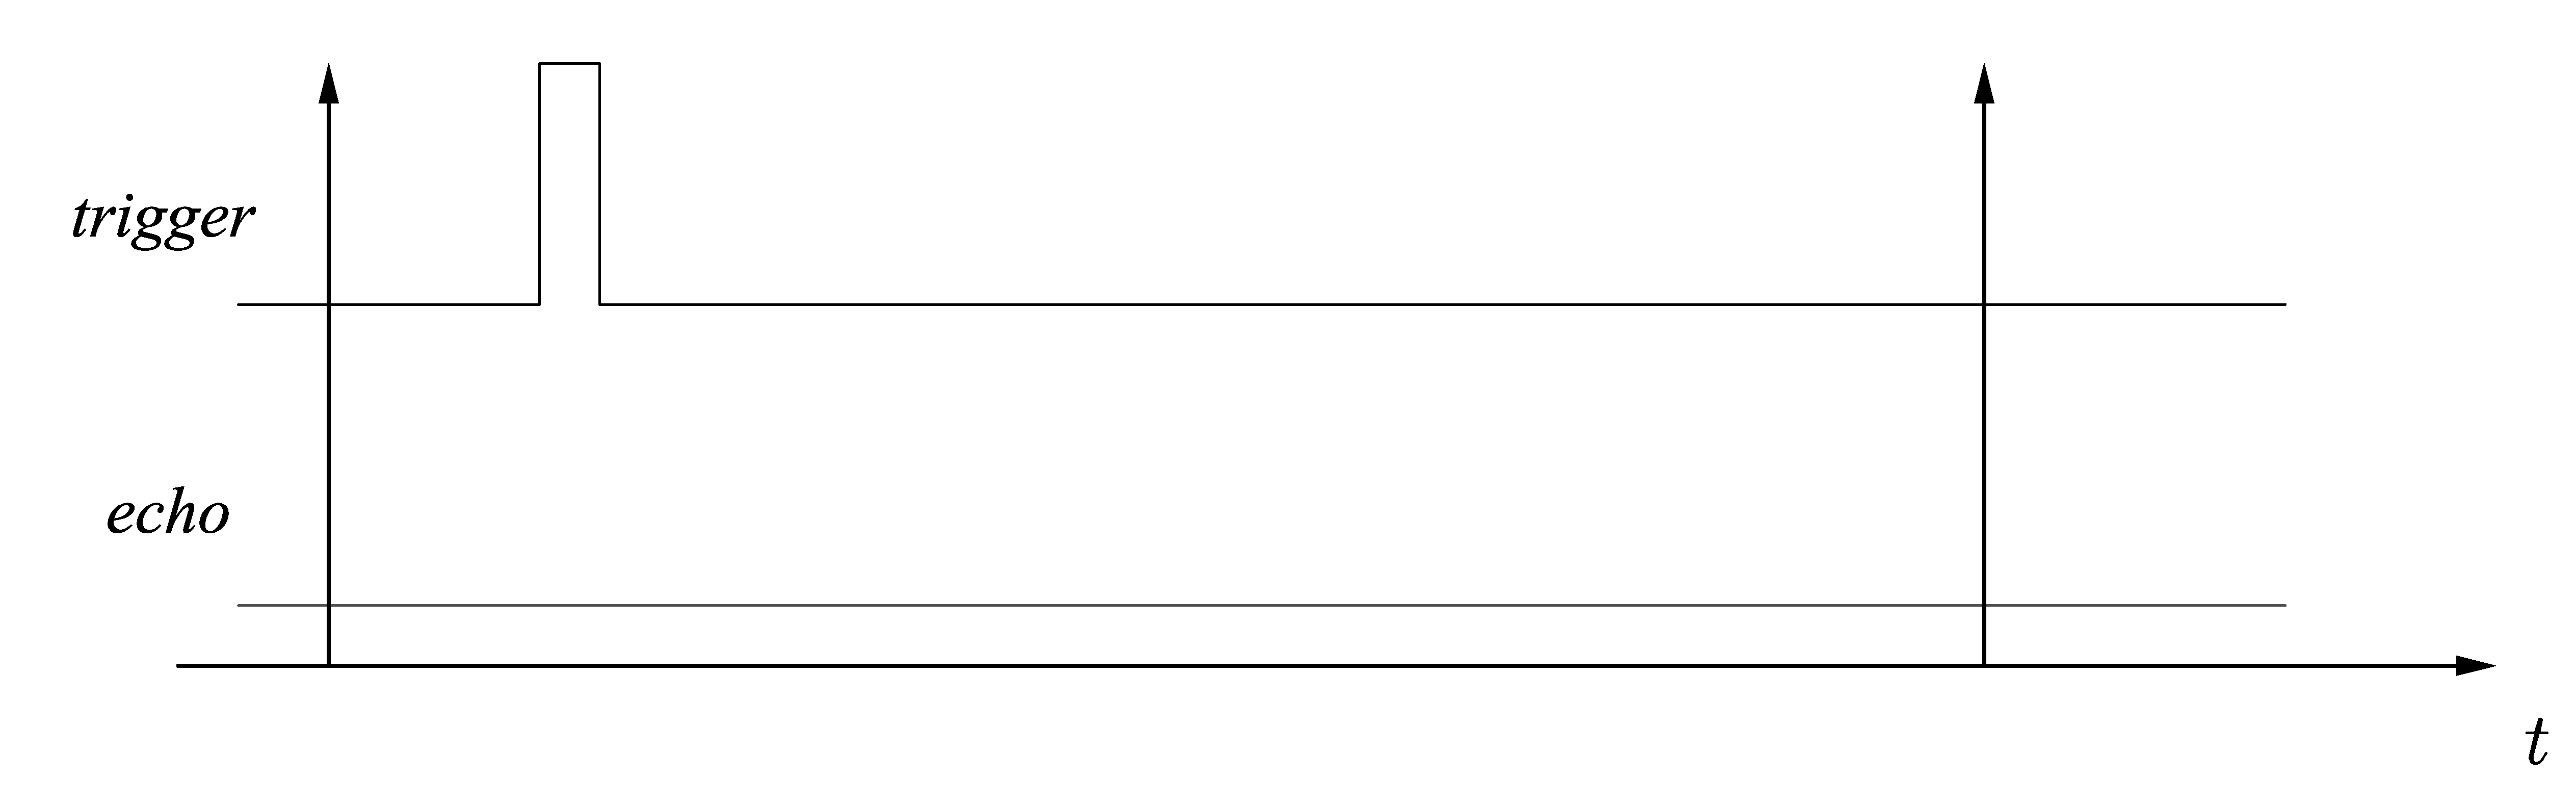
\includegraphics[width=0.8\textwidth]{tikz_img/trig_echo_lost.eps}\label{fig:state_lost}}\\

\subfloat[Stuck at one echo behavior, next state will be State Long and trigger signal will not be sent at next activation]{\includegraphics[width=0.8\textwidth]{tikz_img/trig_echo_long.eps}\label{fig:state_long}}\\

\subfloat[Termination of a stuck at one behavior, next state will be State Next OK and trigger signal can be sent again at next activation]{\includegraphics[width=0.8\textwidth]{tikz_img/trig_echo_next_ok.eps}\label{fig:state_next_ok}}\\
\caption{Various conditions that can be identified by listening to a sensor's echo signal.}
\label{fig:echo_widths}
\end{figure}




Starting from this, possible states in which a system can transition to are:
\begin{description}
    \item[State OK] if echo correctly started and finished within Step Task period;
    \item[State Lost] if echo did not start at all within current period;
    \item[State Long] if echo started within current period, but did not finished;
    \item[State Next OK] if echo started within (one or more) previous period(s), but finished during current period.
\end{description}

When no reply or a too long reply are detected by the system the detected distance is not valid and cannot be shown to the user. Probably a hardware failure made the line getting stuck at either 0 or 1 value. Otherwise, the detected distance is valid.

Obviously, Step Task period must be set in such a way valid distances are not wrongly interpreted as too long ones. To do so, various testings have been made, obtaining the optimal trade-off.

Notice that in the case a sensor's echo line is stuck at a high value, no trigger signal is sent to the sensor, to avoid overlapping of multiple responses altogether. Trigger signals will start to be sent again after the line changes its value again.

The resulting state machine is the one shown in Figure \ref{fig:state_machine}, where for the sake of clarity of the scheme states, inputs and outputs have been translated into integer values. Translation table can be found in Table \ref{tab:state_table}.

\begin{figure}[tp]
\centering
%% MACCHINA A STATI

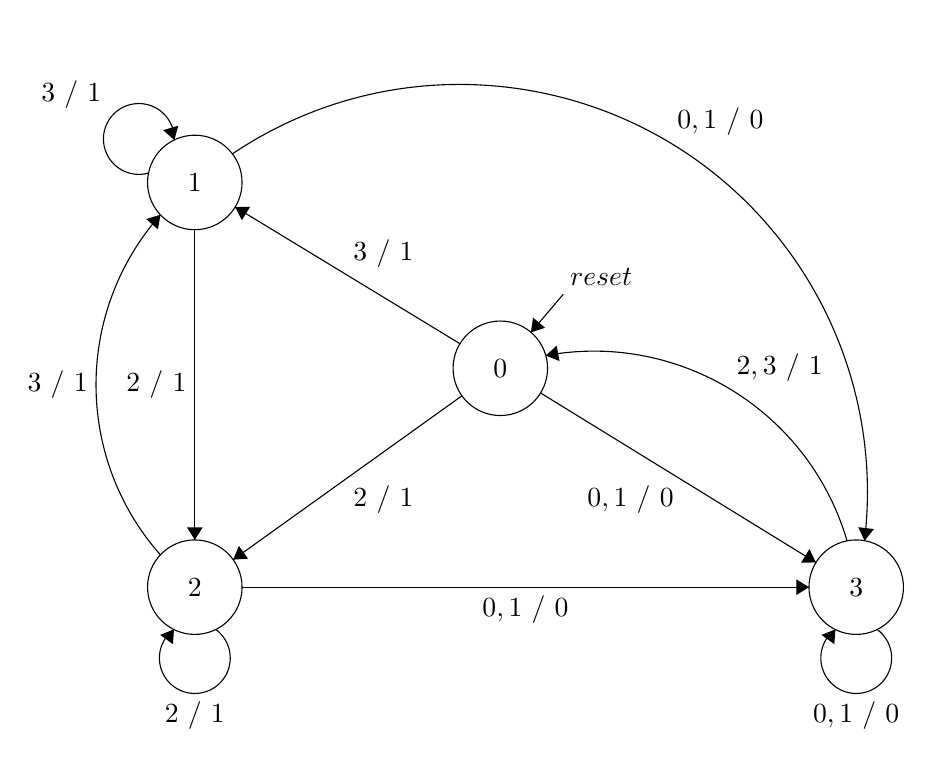
\begin{tikzpicture}[scale=0.2]
\tikzstyle{every node}+=[inner sep=0pt]
\draw [black] (39.9,-27.9) circle (3);
\draw (39.9,-27.9) node {$0$};
\draw [black] (20.5,-16.1) circle (3);
\draw (20.5,-16.1) node {$1$};
\draw [black] (20.5,-41.8) circle (3);
\draw (20.5,-41.8) node {$2$};
\draw [black] (62.5,-41.8) circle (3);
\draw (62.5,-41.8) node {$3$};
\draw [black] (37.34,-26.34) -- (23.06,-17.66);
\fill [black] (23.06,-17.66) -- (23.49,-18.5) -- (24.01,-17.65);
\draw (32.48,-21.5) node [above] {$3\mbox{ }/\mbox{ }1$};
\draw [black] (43.9,-23.2) -- (41.84,-25.62);
\draw (46.3,-22.71) node [above] {$reset$};
\fill [black] (41.84,-25.62) -- (42.74,-25.33) -- (41.98,-24.68);
\draw [black] (17.573,-15.499) arc (286.12502:-1.87498:2.25);
\draw (14.6,-10.54) node [left] {$3\mbox{ }/\mbox{ }1$};
\fill [black] (19.2,-13.41) -- (19.45,-12.5) -- (18.49,-12.78);
\draw [black] (42.46,-29.47) -- (59.94,-40.23);
\fill [black] (59.94,-40.23) -- (59.53,-39.38) -- (59,-40.24);
\draw (48.17,-35.35) node [below] {$0,1\mbox{ }/\mbox{ }0$};
\draw [black] (42.785,-27.093) arc (100.50277:16.31052:16.754);
\fill [black] (42.79,-27.09) -- (43.66,-27.44) -- (43.48,-26.46);
\draw (57.64,-28.79) node [above] {$2,3\mbox{ }/\mbox{ }1$};
\draw [black] (37.46,-29.65) -- (22.94,-40.05);
\fill [black] (22.94,-40.05) -- (23.88,-39.99) -- (23.3,-39.18);
\draw (32.48,-35.35) node [below] {$2\mbox{ }/\mbox{ }1$};
\draw [black] (22.887,-14.285) arc (123.93206:-6.85738:25.881);
\fill [black] (63.03,-38.85) -- (63.62,-38.11) -- (62.63,-37.99);
\draw (53.87,-13.18) node [above] {$0,1\mbox{ }/\mbox{ }0$};
\draw [black] (23.5,-41.8) -- (59.5,-41.8);
\fill [black] (59.5,-41.8) -- (58.7,-41.3) -- (58.7,-42.3);
\draw (41.5,-42.3) node [below] {$0,1\mbox{ }/\mbox{ }0$};
\draw [black] (21.823,-44.48) arc (54:-234:2.25);
\draw (20.5,-49.05) node [below] {$2\mbox{ }/\mbox{ }1$};
\fill [black] (19.18,-44.48) -- (18.3,-44.83) -- (19.11,-45.42);
\draw [black] (18.317,-39.748) arc (-138.50059:-221.49941:16.296);
\fill [black] (18.32,-18.15) -- (17.41,-18.42) -- (18.16,-19.08);
\draw (13.73,-28.95) node [left] {$3\mbox{ }/\mbox{ }1$};
\draw [black] (20.5,-19.1) -- (20.5,-38.8);
\fill [black] (20.5,-38.8) -- (21,-38) -- (20,-38);
\draw (20,-28.95) node [left] {$2\mbox{ }/\mbox{ }1$};
\draw [black] (63.823,-44.48) arc (54:-234:2.25);
\draw (62.5,-49.05) node [below] {$0,1\mbox{ }/\mbox{ }0$};
\fill [black] (61.18,-44.48) -- (60.3,-44.83) -- (61.11,-45.42);
\end{tikzpicture}    
\caption{Erroneous states' state machine}
\label{fig:state_machine}
\end{figure}

\begin{table}[tp]
\centering

\subfloat[States translation table]{%
\begin{tabular}{l|c}%
\hline%
\multicolumn{1}{c|}{\textbf{State Id}} & \textbf{State Label} \\ \hline%
State NEXT OK                          & 0                    \\ %
State OK                               & 1                    \\ %
State LOST                             & 2                    \\ %
State LONG                             & 3                   %
\end{tabular}%
\label{tab:translate_state}%
}
\qquad\qquad
\subfloat[State machine output values]{%
\begin{tabular}{c|c}%
\hline%
\textbf{Send Trigger}   & \textbf{Output Label} \\ \hline%
No                      & 0                     \\ %
Yes                     & 1                     %
\end{tabular}%
\label{tab:translate_output}%
}\\

\subfloat[State machine input values]{%
\begin{tabular}{c|c|c}%
\hline%
\textbf{Echo finished}  & \textbf{Echo started}     & \textbf{Input Label}  \\ \hline%
No                      & Yes                       & 0                     \\ %
No                      & No                        & 1                     \\ %
Yes                     & No                        & 2                     \\ %
Yes                     & Yes                       & 3                     %
\end{tabular}%
\label{tab:translate_input}%
}

\caption{State machine translation tables. Input values are evaluated at Step Task activation.}
\label{tab:state_table}
\end{table}

Given this specification, we need to check whether our software implementation of this state machine is compliant or not with it. To so so, we designed a test suite with complete state and transition coverage usint {\em CUnit}, taking advantage of the fact that we can directly access current state information and set current state directly acting on state machine implementation. Hence, we don't need a {\em transition tour} or more complicated procedures, like {\em PW method}.

Table \ref{tab:conformance} resumes the obtained results, which clearly indicate how our state machine implementation is compliant with the given specification.

%The first test presented in this chapter regard the state-machine that implement the control system of the two sensors. In particular the state-machine was tested using a \textit{conformance test}. The conformance test is one of the most mean fully with respect to state-machine testing. In fact, given a model specification MS, for which the transition diagram is known, and MI, the actual program implementation of MS, with conformance test is possible to check if MI correctly implements MS. The model specification to be tested is the one visible in figure below. This model has been tested using CUnit on the source code of our machine implementation.


%% FSM Conformance TEST

\begin{table}[tp]
\centering

\subfloat[Conformance test suite tests]{%
\begin{tabular}{cl|c|c}%
\hline%
                           &                               & \textbf{Test Count} & \textbf{Active?} \\ \hline%
\multicolumn{1}{c|}{Suite} & \textbf{FSM Conformance Test} & 4                   & Yes              \\ \hline%
\multicolumn{1}{c|}{Test}  & State NEXT\_OK                &                     & Yes              \\%
\multicolumn{1}{c|}{Test}  & State OK                       &                     & Yes              \\%
\multicolumn{1}{c|}{Test}  & State LOST                    &                     & Yes              \\%
\multicolumn{1}{c|}{Test}  & State LONG                    &                     & Yes             
\end{tabular}%
\label{tab:conf_suite_test}%
}\\


\subfloat[Tests outcomes]{%
\begin{tabular}{l|c}%
\hline%
\textbf{Running Suite FSM Conformance Test} & \textbf{Outcome} \\ \hline%
Running test State NEXT\_OK                 & Passed           \\%
Running test State OK                       & Passed           \\%
Running test State LOST                     & Passed           \\%
Running test State LONG                     & Passed          %
\end{tabular}%
\label{tab:conf_outcome}%
}\\

\caption{FSM conformance test suite and results.}
\label{tab:conformance}
\end{table}





\section{Functional Tests}

The second suite that we defined performs functional testing on the implementation of the triangulation function, which is used to determine actual distance of a detected obstacle based on the distances measured by the two distinct sensors. To do so, we considered the function as a black box and determined test values by simply looking at expected input variables ranges and types.

Table \ref{tab:functional} resumes the obtained results, from which we can clearly detect that there was an error handling some out-of-range values of input variables, since robustness tests failed. Thanks to the test, we could detected easily the error and fix it. Test results on the fixed software can be found in Table \ref{tab:functional2}.


\begin{table}[tp]
\centering

\subfloat[Triangulation functional test suite tests]{%
\begin{tabular}{cl|c|c}%
\hline%
                           &                                           & \textbf{Test Count} & \textbf{Active?} \\ \hline%
\multicolumn{1}{c|}{Suite} & \textbf{Triangulation Functional Testing} & 6                   & Yes              \\ \hline%
\multicolumn{1}{c|}{Test}  & Nominal Testing                           &                     & Yes              \\%
\multicolumn{1}{c|}{Test}  & Boundary Testing                          &                     & Yes              \\%
\multicolumn{1}{c|}{Test}  & Robustness Testing                        &                     & Yes              \\%
\multicolumn{1}{c|}{Test}  & Worst-Case Testing                        &                     & Yes              \\%
\multicolumn{1}{c|}{Test}  & Worst-Case Robustness Testing             &                     & Yes              \\%
\multicolumn{1}{c|}{Test}  & Random Testing                            &                     & Yes             %
\end{tabular}%
\label{tab:func_suite_test}%
}\\


\subfloat[Tests outcomes]{%
\begin{tabular}{l|c}%
\hline%
\textbf{Running Suite Triangulation Functional Testing} & \textbf{Outcome} \\ \hline%
Running test Nominal Testing                            & Passed           \\%
Running test Boundary Testing                           & Passed           \\%
Running test Robustness Testing                         & \textbf{Failed}  \\%
Running test Worst-Case Testing                         & Passed           \\%
Running test Worst-Case Robustness Testing              & \textbf{Failed}  \\%
Running test Random Testing                             & Passed          %
\end{tabular}%
\label{tab:func_outcome}%
}\\

\caption{Triangulation functional test suite and initial results.}
\label{tab:functional}
\end{table}





\begin{table}[tp]
\centering
\begin{tabular}{l|c}
\hline
\textbf{Running Suite Fixed Triangulation Functional Testing} & \textbf{Outcome} \\ \hline
Running test Nominal Testing                                  & Passed           \\
Running test Boundary Testing                                 & Passed           \\
Running test Robustness Testing                               & Passed           \\
Running test Worst-Case Testing                               & Passed           \\
Running test Worst-Case Robustness Testing                    & Passed           \\
Running test Random Testing                                   & Passed          
\end{tabular}
\caption{Fixed triangulation functional test suite outcomes.}
\label{tab:functional2}
\end{table}

Table \ref{tab:cumulative} shows cumulative results for both illustrated test suites.

\begin{table}[tp]
\centering
\begin{tabular}{cccccc}
\multicolumn{6}{c}{\textbf{Cumulative Summary for Run}}                                                                                                                                                          \\ \hline
\multicolumn{1}{c|}{\textbf{Type}} & \multicolumn{1}{c|}{\textbf{Total}} & \multicolumn{1}{c|}{\textbf{Run}} & \multicolumn{1}{c|}{\textbf{Succeeded}} & \multicolumn{1}{c|}{\textbf{Failed}} & \textbf{Inactive} \\ \hline
\multicolumn{1}{c|}{Suites}        & \multicolumn{1}{c|}{2}              & \multicolumn{1}{c|}{2}            & \multicolumn{1}{c|}{- NA -}            & \multicolumn{1}{c|}{0}               & 0                 \\
\multicolumn{1}{c|}{Test Cases}    & \multicolumn{1}{c|}{10}             & \multicolumn{1}{c|}{10}           & \multicolumn{1}{c|}{10}                & \multicolumn{1}{c|}{0}               & 0                 \\
\multicolumn{1}{c|}{Assertions}    & \multicolumn{1}{c|}{83}             & \multicolumn{1}{c|}{83}           & \multicolumn{1}{c|}{83}                & \multicolumn{1}{c|}{0}               & N/A              
\end{tabular}
\caption{Cumulative outcomes summary for the all test suites.}
\label{tab:cumulative}
\end{table}

\section{Tests coverage}

We also proved actual goodness of these test suites calculating also coverage of automatic testing code. To do so, we used {\em GCov} suite in combination with {\em CUnit} to obtain code lines execution statistics. In order to summarize these stats, we used {\em LCov} suite, which takes {\em GCov} results and creates with them HTML pages containing both cumulative results and individual lines stats.

Thanks to these tools, we proved that our tests cover 100\% of tested code, hence proving their goodness. This result is shown in Table \ref{tab:coverage}.


% The last part of testing chapter present test coverage results calculated using \textit{gcov}, an open source and free tool from the gnu foundation. Gcov is a test coverage program that is meant to be used in concert with gcc to analyze programs and discover untested parts of it. Gcov creates a log file which indicates how many times each line of a source file has executed. In order to make the gcov report readable, another tool called lcov can be used. Lcov is a graphical front-end for gcov, it collects gcov data for multiple source files and creates HTML pages containing the source code annotated with coverage information. The results of coverage test show that 100\% of test code lines are executed.


\begin{table}[htp]
\centering
\begin{tabular}{c|ccc|cc}
\hline
\textbf{Filename} & \multicolumn{3}{c|}{\textbf{Lines Coverage}} & \multicolumn{2}{c}{\textbf{Functions}} \\ \hline
main.c            
& 
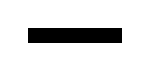
\begin{tikzpicture}
      \fill[black] (0,0) rectangle (1.2,0.2) ;
\end{tikzpicture}
& 100.0\%       & 168/168       & 100.0\%             & 18/18             \\
sensor.c          
&
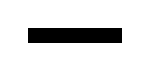
\begin{tikzpicture}
      \fill[black] (0,0) rectangle (1.2,0.2) ;
    \end{tikzpicture}
& 100.0\%       & 35/35         & 100.0\%             & 3/3              
\end{tabular}
\caption{Cumulative stats obtained by checking coverage of given test suites.}
\label{tab:coverage}
\end{table}






%% TODO




% As most software tend to grow in complexity over time, it becomes increasingly difficult to test. In the same way of software that itself needs to be broken into more manageable units, so do the tests. As the new units are developed, it makes sense to consider adding automated unit tests, where each unit is isolated and tested out of its context. Our text has built using \textit{CUnit} that is a lightweight system for writing, administering, and running unit tests in C.  It provides C programmers a basic testing functionality with a flexible variety of user interfaces. By means of CUnit, two different suite of tests were been executed. The first test-suite is a conformance test, the second a black box functional test.

% The second suite of test registered and executed by CUnit regards the implementation of the triangulation function. The triangulation function was used to elaborate data received by the two sensors separately and to calculate the correct position of objects. In functional testing the main assumption is that software or system to be examined is a function from inputs to outputs. The registered tests give an input to the system and check if the actual output is the expected one. The input used to test the software are predefined and chosen accordingly to the test-method.